\chapter{Diagramas adicionales}

\section{Diagramas de flujo de la plataforma}

Este anexo complementa el Capítulo 6 (Plataforma web en la nube) presentando los diagramas de flujo y arquitectura interna de los tres componentes principales que conforman la plataforma: el frontend de aplicación de página única, el backend de servicios y orquestación, y el servicio de postprocesamiento para análisis espectral. Estos diagramas detallan la estructura interna, los flujos de datos y las interacciones entre los módulos que componen cada uno de estos componentes.

\subsection{Frontend}

El frontend de la plataforma web está desarrollado con React 19, TypeScript y Vite. El siguiente diagrama presenta la organización de componentes, el flujo de navegación entre pantallas y las conexiones con los servicios externos: API REST mediante Axios, WebSocket para datos en tiempo real y streaming de audio demodulado.

\begin{figure}[H]
    \centering
    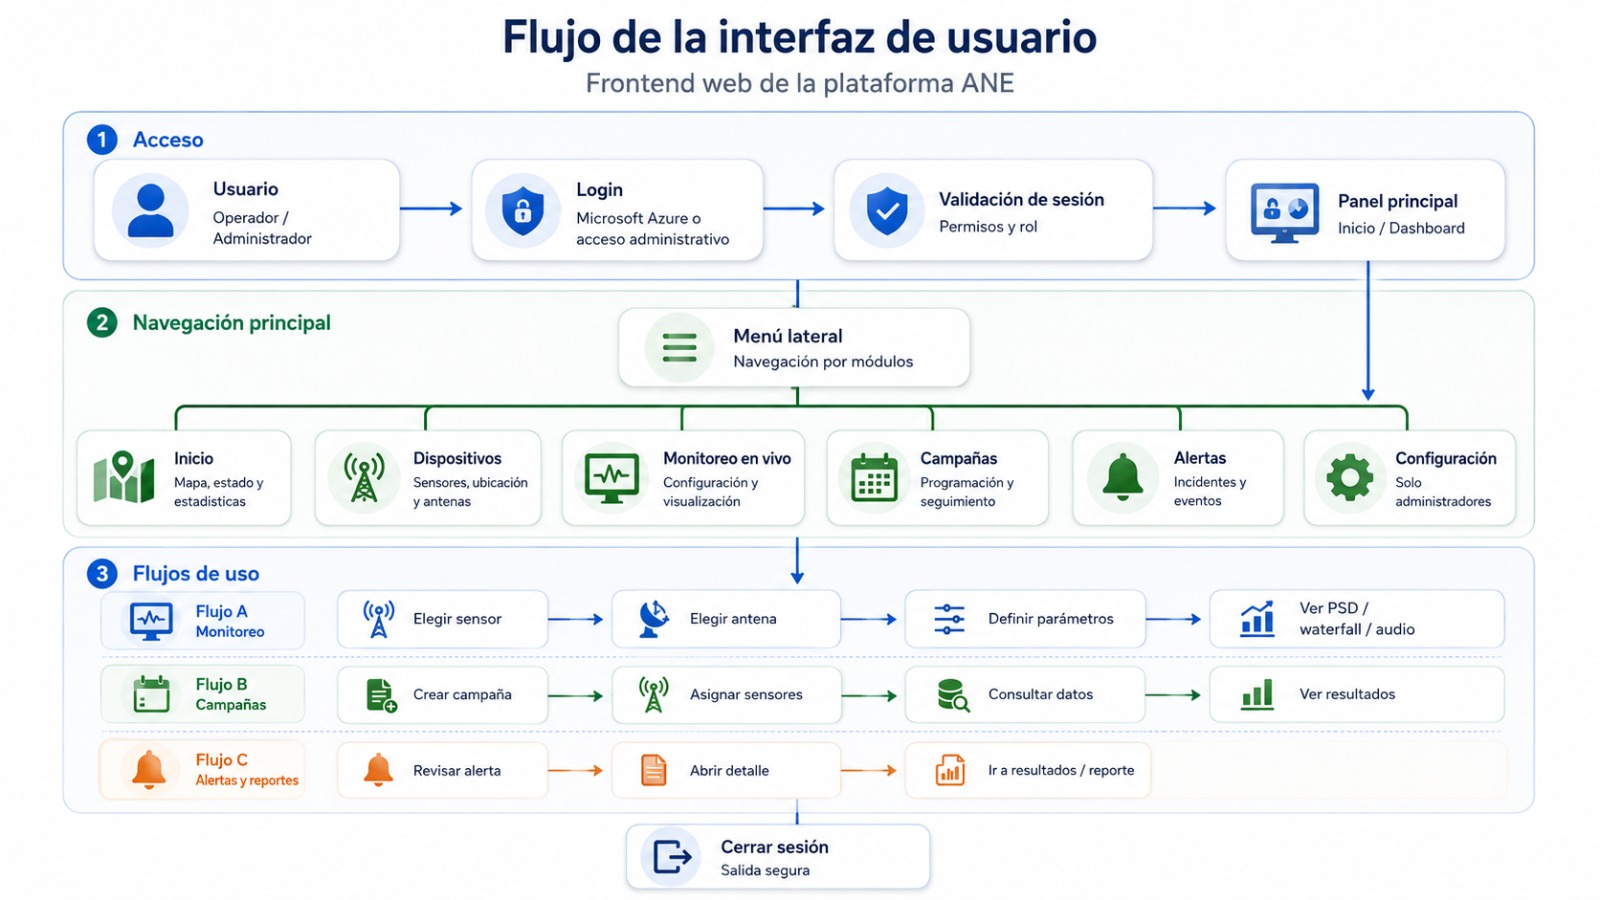
\includegraphics[width=0.85\textwidth]{section/img/annexes/FRONTEND-diagram.jpeg}
    \caption{Diagrama de arquitectura y flujo del frontend de la plataforma web. Fuente: Elaboración propia.}
    \label{fig:frontend_diagram}
\end{figure}

\subsection{Backend}

El backend implementa un servidor Node.js con Express y TypeScript, organizado en seis capas lógicas. El diagrama a continuación ilustra la arquitectura interna del backend, incluyendo las capas de entrada HTTP, autenticación y autorización, rutas y controladores, modelos de acceso a datos, comunicación en tiempo real mediante WebSocket y las tareas de mantenimiento automático.

\begin{figure}[H]
    \centering
    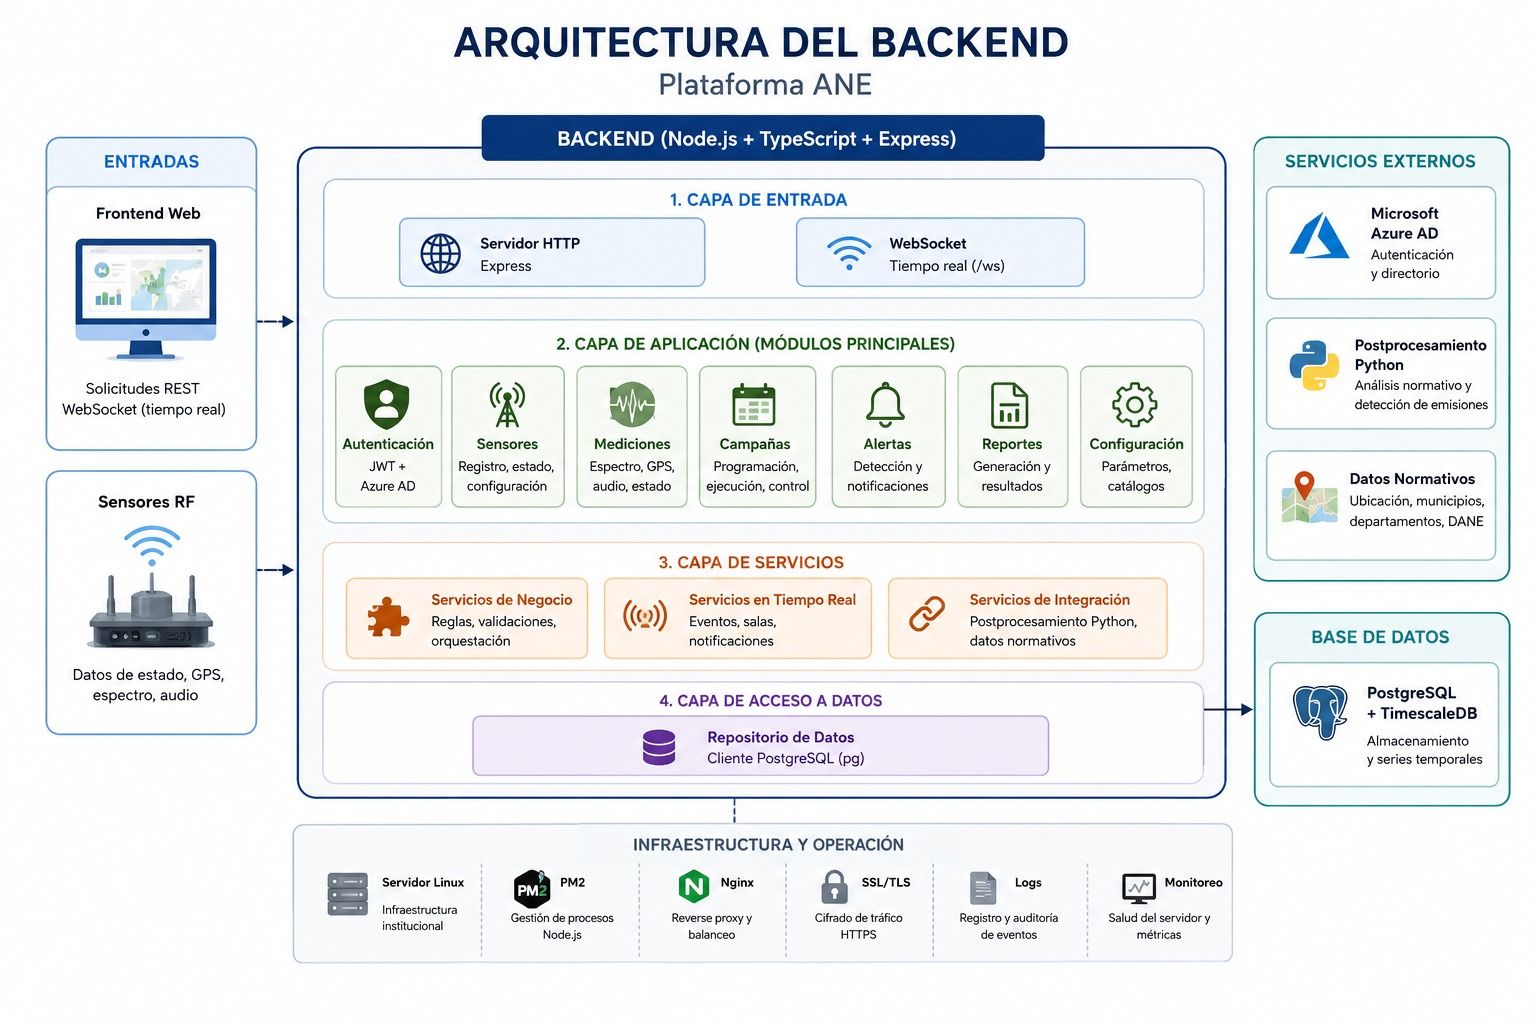
\includegraphics[width=0.85\textwidth]{section/img/annexes/BACKEND-diagram.jpeg}
    \caption{Diagrama de arquitectura y flujo del backend de la plataforma web. Fuente: Elaboración propia.}
    \label{fig:backend_diagram}
\end{figure}

\subsection{Postprocesamiento}

El servicio de postprocesamiento es un microservicio independiente implementado en Python con Flask, responsable del análisis espectral avanzado. El siguiente diagrama muestra el flujo de procesamiento desde la recepción de datos espectrales hasta la generación de resultados de análisis, incluyendo la detección de emisiones, la estimación del piso de ruido, el cruce con la base de datos de licencias y la evaluación de cumplimiento normativo.

\begin{figure}[H]
    \centering
    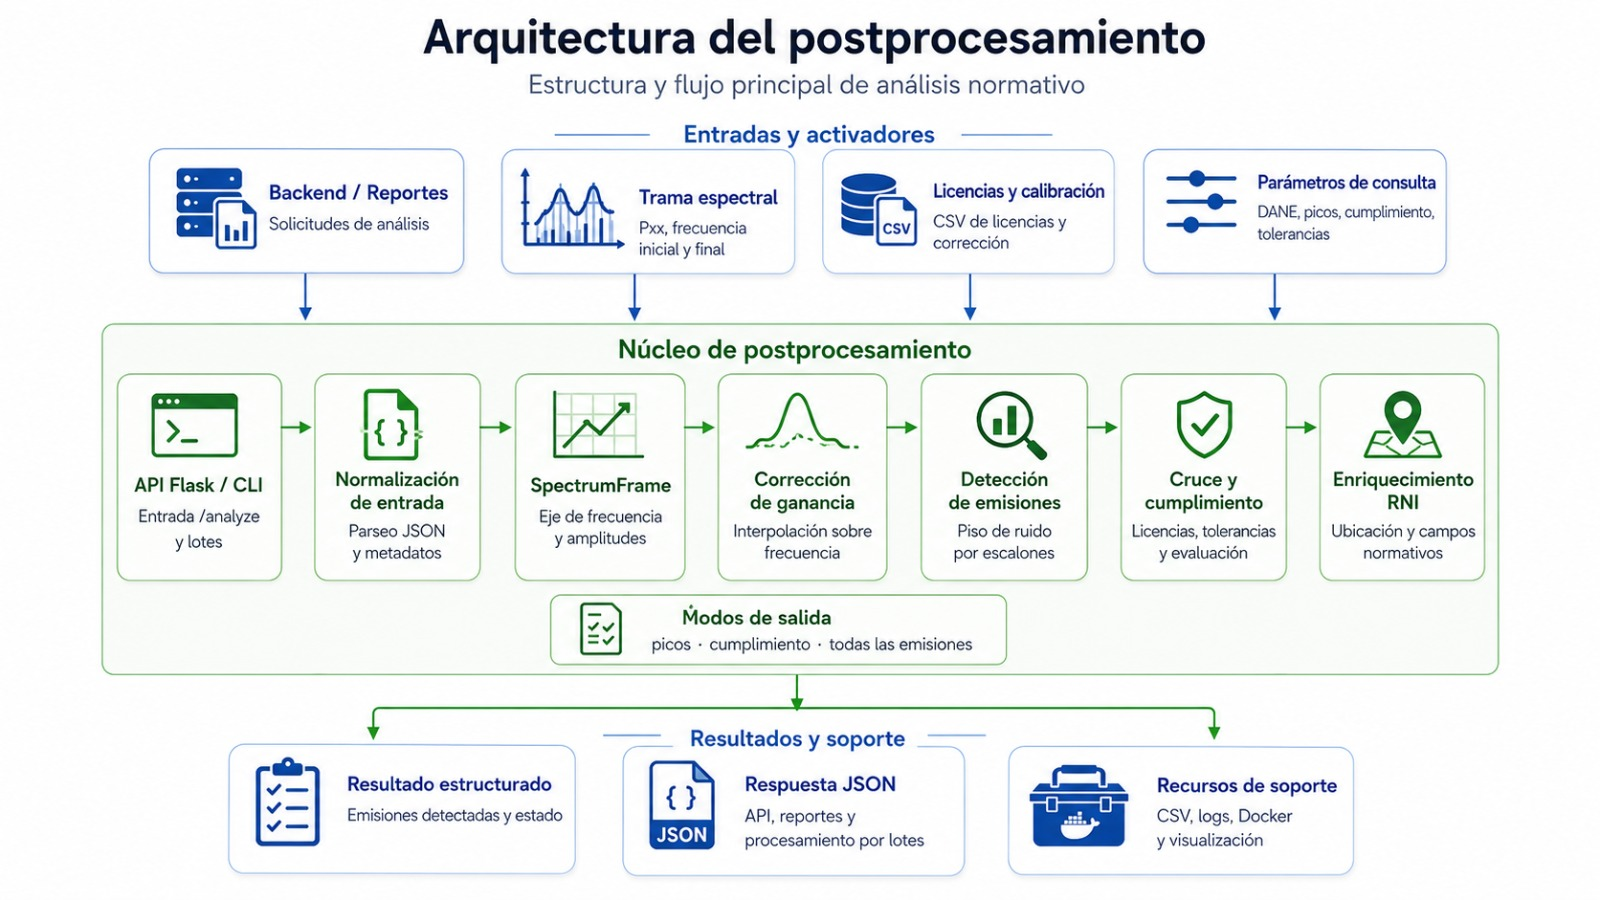
\includegraphics[width=0.85\textwidth]{section/img/annexes/POTPROCESAMIENTO-diagram.jpeg}
    \caption{Diagrama de arquitectura y flujo del servicio de postprocesamiento. Fuente: Elaboración propia.}
    \label{fig:postprocesamiento_diagram}
\end{figure}

\section{Diagramas de despliegue y conectividad}
[[Placeholder]]

\section{Secuencias operativas}
[[Placeholder]]

\section{Esquemas detallados de componentes}
[[Placeholder]]
